\documentclass[11pt,a4paper]{article}
\usepackage[margin=2.2cm]{geometry}
\usepackage{booktabs}
\usepackage{array}
\usepackage{xcolor}
\usepackage{titlesec}
\usepackage{enumitem}
\usepackage{graphicx}
\usepackage{subcaption}
\usepackage{hyperref}
\hypersetup{colorlinks=true, linkcolor=blue!50!black, urlcolor=blue!50!black}

\titleformat{\section}{\Large\bfseries}{\thesection.}{0.5em}{}
\titleformat{\subsection}{\large\bfseries}{\thesubsection}{0.5em}{}

\title{\textbf{Paper 1 Progress Update} \\
\large BLG vs $\beta$-Casein Comparative Study at the Air--Water Interface}
\author{Chalakon Pornjariyawatch}
\date{September 11, 2026 \\ \small Prepared for: Prapasiri Pongprayoon}

\begin{document}
\maketitle

\section*{Executive Summary}
\begin{itemize}[leftmargin=1.5em]
  \item \textbf{BLG dataset is complete and internally consistent} across 4 independent
  replicas (4.00 $\mu$s total unbiased MD). All four show a stable, compact fold
  (radius of gyration 1.49--1.50 nm) with no evidence of structural commitment upon
  contact with the interface.
  \item \textbf{CASEIN now has its second independent replicate (R1) for the first time},
  alongside the original CENTER run -- all 7 planned analyses complete on both. The
  N-terminal region's solvent accessibility reproduces tightly across the two replicas
  (24.8--25.4 nm$^2$), strengthening the "open chain" comparative claim.
  \item \textbf{The comparative headline holds up with real replication now:} BLG's calyx
  stays small and selectively accessible (3.15--3.81 nm$^2$), while CASEIN's N-terminus is
  both far larger and almost permanently exposed (contact in 99.5\% of frames, in both
  CENTER and R1) -- consistent with "An Accessible Calyx and an Open Chain."
  \item \textbf{Surface tension cross-validates across species and replicas} (BLG
  $\approx$52 mN/m, CAS $\approx$52 mN/m), matching the TIP3P water model's literature
  value ($\approx$50--52 mN/m) -- a good internal consistency check on both force fields.
  \item \textbf{One data-completeness issue found and being corrected:} three of BLG's four
  replicas were run in multiple simulation segments; for two analyses ($R_g$ and surface
  tension), the current scripts only read the first segment (500 of 1000 ns) for those
  three replicas. RMSD and calyx SASA already read the full 1000 ns for all replicas.
  This does not invalidate the existing results -- values are internally consistent and match previously reported
  numbers -- but the per-replica table below should be read with that caveat until the fix
  lands (see note under Table 1).
\end{itemize}

\begin{figure}[h]
\centering
\begin{subfigure}{0.45\textwidth}
\centering
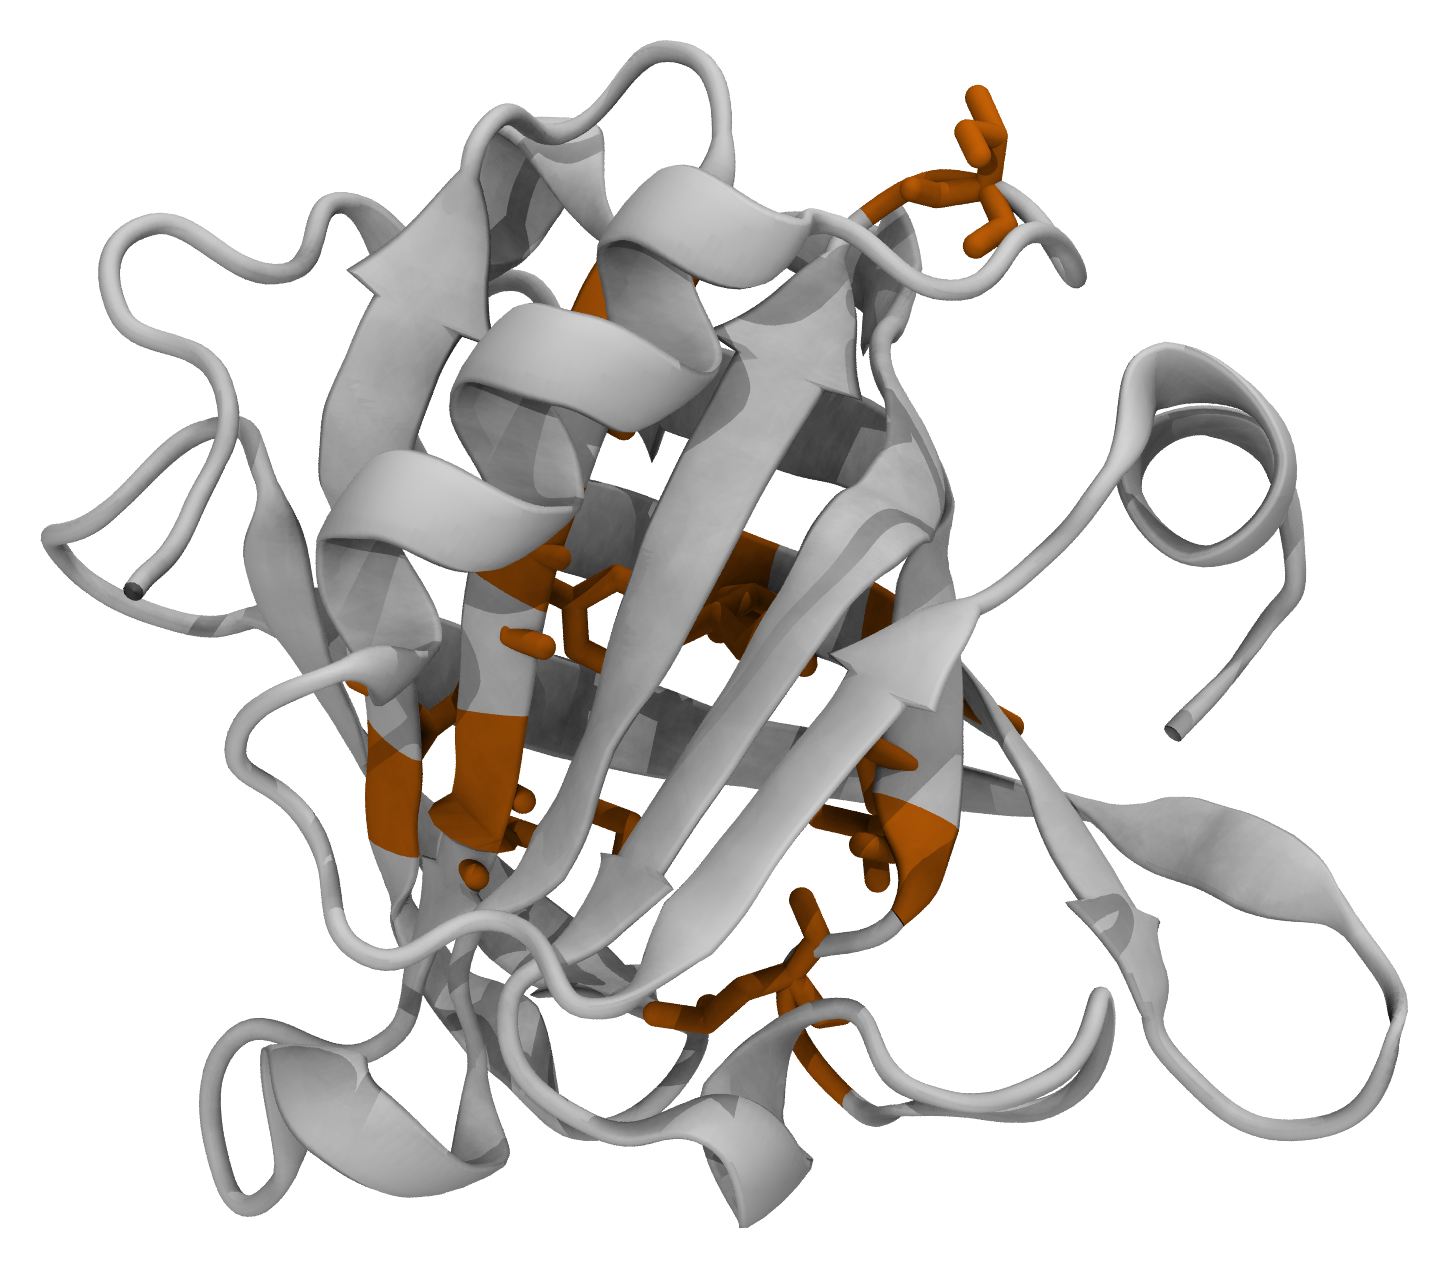
\includegraphics[width=\textwidth]{../results/figures/render/blg_calyx_crop.png}
\caption{BLG: compact fold, calyx patch (orange)}
\end{subfigure}
\hfill
\begin{subfigure}{0.45\textwidth}
\centering
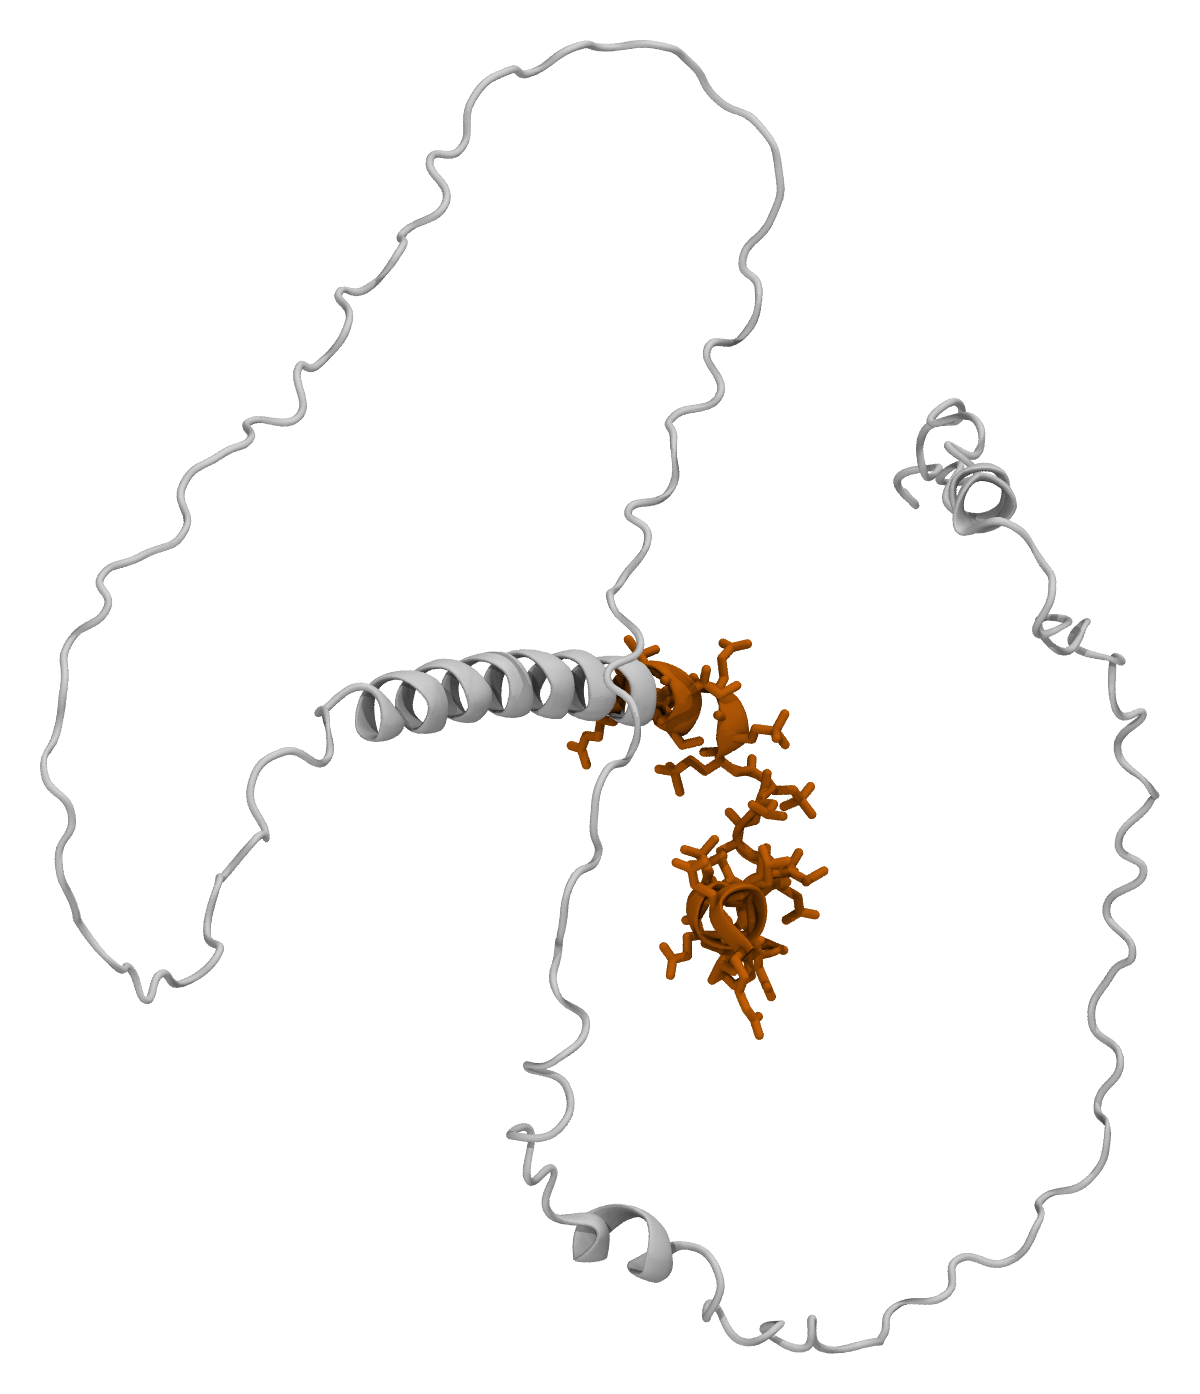
\includegraphics[width=\textwidth]{../results/figures/render/cas_patch_crop.png}
\caption{CASEIN: extended chain, N-term (orange)}
\end{subfigure}
\caption{Structural contrast between the two proteins (VMD renders): BLG's compact,
mostly-buried calyx vs. CASEIN's extended, disordered chain with its N-terminal region
already surface-exposed even in the starting structure.}
\end{figure}

\section{BLG Results}

\textbf{Headline numbers (unchanged, PBC-corrected, computed across all 4 replicas):}
613 total contact events (97 in CENTER, 516 near-interface across replicas); 6 long
contact events ($\geq$10 ns); calyx SASA range 24--37 nm$^2$ (mean 28.95 nm$^2$); Pearson
correlation between SASA and orientation angle $r = +0.006$ (block-bootstrap 95\% CI
$[-0.09, +0.11]$) -- no coupling detected within these limits. These support the paper's
current framing: BLG's calyx remains accessible throughout, but the protein does not
commit to a bound, reoriented state within the simulated timescale.

\begin{table}[h]
\centering
\scriptsize
\setlength{\tabcolsep}{4pt}
\begin{tabular}{lccccc}
\toprule
Replica & $R_g$ (nm)$^*$ & RMSD bb (nm) & RMSD patch (nm) & Calyx SASA (nm$^2$) & $\gamma$ (mN/m)$^*$ \\
\midrule
CENTER (1000 ns) & 1.504 $\pm$ 0.022 & 0.229 & 0.198 & 3.81 $\pm$ 0.46 & 51.9 $\pm$ 38.5 \\
R1                & 1.497 $\pm$ 0.009 & 0.237 & 0.347 & 3.15 $\pm$ 0.34 & 52.7 $\pm$ 38.7 \\
R2                & 1.493 $\pm$ 0.008 & 0.206 & 0.254 & 3.59 $\pm$ 0.32 & 52.0 $\pm$ 39.0 \\
R3                & 1.499 $\pm$ 0.012 & 0.268 & 0.276 & 3.36 $\pm$ 0.48 & 52.6 $\pm$ 39.4 \\
\bottomrule
\end{tabular}
\normalsize
\caption{BLG per-replica structural summary. $^*$For R1/R2/R3, only $R_g$ and $\gamma$
(surface tension) currently reflect the first 500 of 1000 ns each replica actually ran
-- a fix to include the remaining trajectory segments for these two analyses is in
progress. RMSD and calyx SASA for R1/R2/R3 already cover the full 1000 ns (their
analysis scripts already include the extension trajectory segments).}
\end{table}

Secondary structure content (DSSP) is stable across all 4 replicas: Helix 10.5--12.4\%,
Sheet 36.0--36.8\%, Coil 50.8--52.9\%. Hydrogen-bonding (CENTER only so far):
protein--protein 107.3 $\pm$ 5.6, protein--water 393.2 $\pm$ 13.2, interface
water--water 9539.6 $\pm$ 328.4 (mean counts per frame).

\section{CASEIN ($\beta$-casein) Results}

\textbf{First comparative result with real replication (n=2):} N-terminal region (residues
1--25) solvent accessibility -- the CASEIN analogue of BLG's calyx SASA -- is
24.77 $\pm$ 1.40 nm$^2$ in R1 vs. 25.41 $\pm$ 1.97 nm$^2$ in CENTER. The two independent
1000 ns runs agree closely, which is good evidence this is a real, reproducible property
of the protein rather than an artifact of one starting structure.

\begin{table}[h]
\centering
\scriptsize
\setlength{\tabcolsep}{4pt}
\begin{tabular}{lccccc}
\toprule
Replica & N-term SASA (nm$^2$) & Contact & $\gamma$ (mN/m) & Hbonds prot-prot & Hbonds prot-water \\
\midrule
CENTER (1000 ns) & 25.41 $\pm$ 1.97 & 99.5\% & 51.4 $\pm$ 34.2 & 97.8 $\pm$ 9.7 & 565.5 $\pm$ 25.1 \\
R1 (1000 ns)     & 24.77 $\pm$ 1.40 & 99.5\% & 52.4 $\pm$ 34.6 & 92.0 $\pm$ 8.3 & 575.9 $\pm$ 24.0 \\
\bottomrule
\end{tabular}
\normalsize
\caption{CASEIN per-replica summary. Both replicas now have all 7 planned analyses
complete; R1's hydrogen-bonding analysis is the most recently finished. "Contact" is
the fraction of frames with a protein-water minimum distance $\leq$0.3 nm; R1 shows 1
sustained contact event across the full 1000 ns run.}
\end{table}

\begin{figure}[h]
\centering
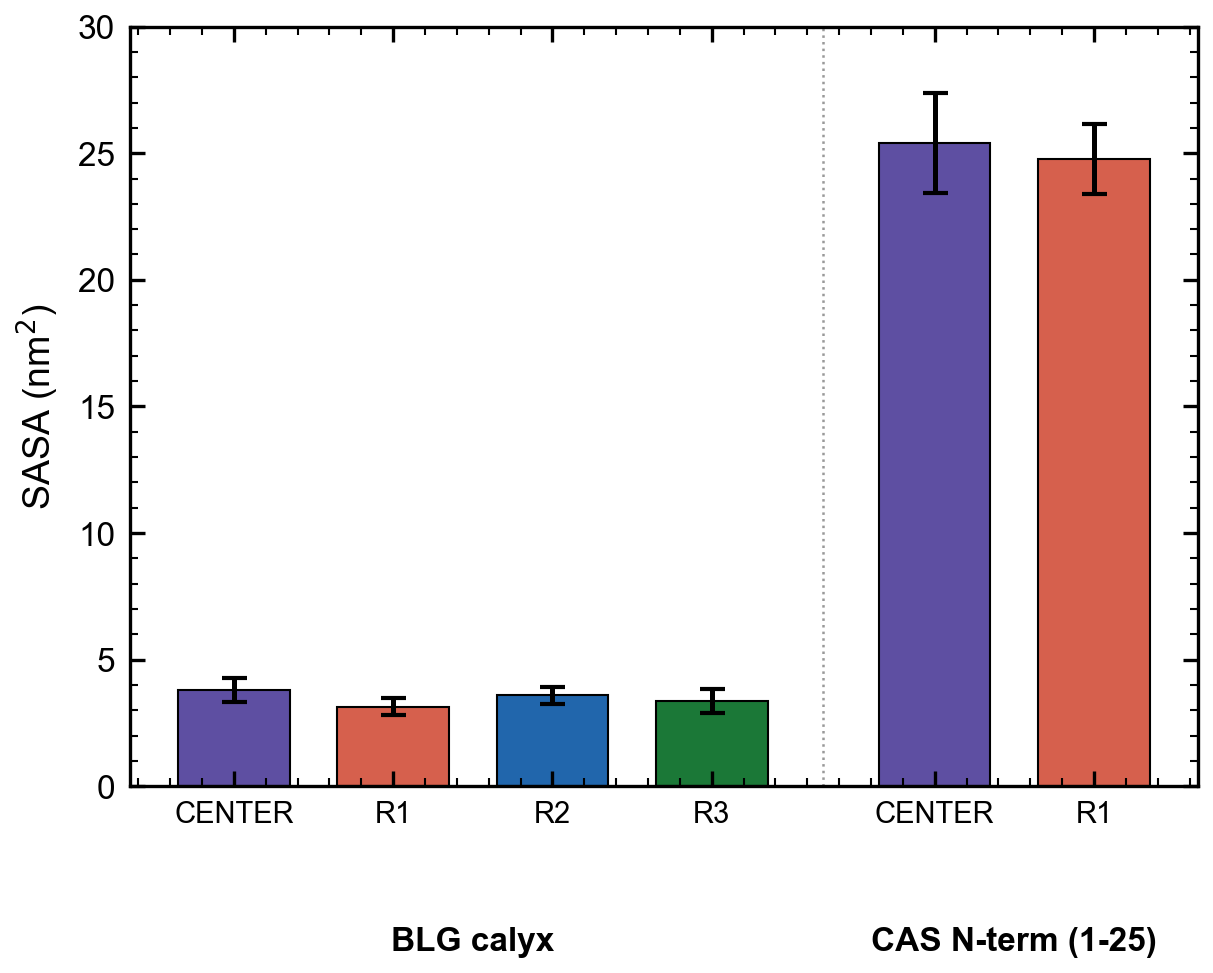
\includegraphics[width=0.62\textwidth]{../results/figures/paper/PAPER_COMPARATIVE_SASA.png}
\caption{Accessible surface area, BLG calyx vs. CASEIN N-terminal region (residues
1--25), all replicas. The $\sim$7-fold size difference is consistent across every
replica of both proteins -- not an artifact of any single run.}
\end{figure}

CASEIN's near-constant interfacial contact (99.5\% of frames in \emph{both} CENTER and R1,
versus BLG's much more selective, intermittent contact pattern across 4$\mu$s) is a clear
structural contrast that
directly supports the comparative title: BLG presents a small, selectively-accessible
calyx, while CASEIN's disordered chain stays persistently near the interface with its
N-terminal region continuously exposed. Rg for R1 confirms the same relaxation pattern
already seen in CENTER: an initial compaction from the extended AlphaFold starting
structure ($\sim$2.85 nm in the first 100 ns) settling to a stable range ($\sim$2.5 nm)
for the remainder of the trajectory -- reassuring that this is a real, reproducible
relaxation, not a one-off artifact of the CENTER run's starting conformation.
Hydrogen-bonding is also now complete for both replicas and agrees closely
(protein-protein 92.0--97.8, protein-water 565.5--575.9, interface water-water
12015.6--12750.5 mean counts per frame) -- another independent confirmation that
CENTER's behavior was not a one-off.

\section{Questions for P.P.}

\begin{enumerate}[leftmargin=1.5em]
  \item \textbf{IFSC2026 (time-sensitive) --} the abstract deadline is Sept 25, 2026 --
  \textbf{14 days away as of this report.} We still have no confirmation whether
  participation is actually happening, or which framing (BLG-only complete story vs.
  BLG+CAS-in-progress) you'd prefer for the poster. This needs an answer this week to
  leave time to draft the abstract.
  \item \textbf{"Secondary SASA" definition --} your June 9 note is ambiguous between
  per-secondary-structure-element SASA (computable now) and a $\Delta$SASA-on-adsorption
  (not computable -- no completed adsorption event exists in either dataset). We propose
  the former; a one-line confirmation from you would let us build it.
  \item \textbf{Lab experiment correlation --} should the "correlation with lab experiment"
  comparison be against published literature (already surveyed) or in-house wet-lab data?
  We see no evidence of in-house tensiometry capability in the group, so we're assuming
  literature -- please confirm.
  \item \textbf{How prescriptive should the "modify to adsorb" claim be?} We have
  data supporting a soft design-principle statement (disorder + exposed hydrophobic
  patches lower the kinetic barrier to adsorption), but not a strong causal claim, since
  neither dataset shows a completed adsorption event. Please confirm this is the right
  level of claim for Paper 1.
  \item \textbf{Co-author review of the BLG-only draft} -- still the hard blocker for
  eventual submission. Whenever you have time for a pass, we're ready.
\end{enumerate}

\vspace{1em}
\noindent\small \textit{Note: all numbers above are PBC-corrected and read directly from
current result files as of this report's generation date -- treat as current, not frozen,
if analysis is rerun later.}

\end{document}
